%; whizzy document
% latex beamer presentation.
% platex, latex-beamer でコンパイルすることを想定。 

%     Tokyo Debian Meeting resources
%     Copyright (C) 2007 Junichi Uekawa

%     This program is free software; you can redistribute it and/or modify
%     it under the terms of the GNU General Public License as published by
%     the Free Software Foundation; either version 2 of the License, or
%     (at your option) any later version.

%     This program is distributed in the hope that it will be useful,
%     but WITHOUT ANY WARRANTY; without even the implied warranty of
%     MERCHANTABILITY or FITNESS FOR A PARTICULAR PURPOSE.  See the
%     GNU General Public License for more details.

%     You should have received a copy of the GNU General Public License
%     along with this program; if not, write to the Free Software
%     Foundation, Inc., 51 Franklin St, Fifth Floor, Boston, MA  02110-1301 USA

% 実行順番
% sudo  ~/bin/usb-macbook-ir.c &
% real presentation (shell-command (concat "DISPLAY=:0.1 xpdf -fullscreen " (replace-regexp-in-string "tex$" "pdf"(buffer-file-name)) "&"))
% DISPLAY=:0.1 xpdf -fullscreen 

\documentclass[cjk,dvipdfmx,12pt]{beamer}
\usetheme{Tokyo}

%  preview (shell-command (concat "xpdf " (replace-regexp-in-string "tex$" "pdf"(buffer-file-name)) "&"))
%  presentation (shell-command (concat "xpdf -fullscreen " (replace-regexp-in-string "tex$" "pdf"(buffer-file-name)) "&"))

%http://www.naney.org/diki/dk/hyperref.html
%日本語EUC系環境の時
\AtBeginDvi{\special{pdf:tounicode EUC-UCS2}}
%シフトJIS系環境の時
%\AtBeginDvi{\special{pdf:tounicode 90ms-RKSJ-UCS2}}

\title{10:45- Debian 紹介}
\subtitle{Linux World Expo/Tokyo 2007}
\author{Debian JP Project 上川 純一}
\date{2007年6月1日}
\logo{
\includegraphics[width=8cm]{image200607/openlogo-light.eps}}


% 三択問題用
\newcounter{santakucounter}
\newcommand{\santaku}[5]{%
\addtocounter{santakucounter}{1}
\frame{\frametitle{問題\arabic{santakucounter}. #1}
%問題\arabic{santakucounter}. #1
\begin{minipage}[t]{0.8\hsize}
 \begin{itemize}
 \item
      \begin{minipage}{0.2\hsize}
      
\includegraphics[width=0.9\hsize]{image200703/janken-A.png}\end{minipage} 
       \begin{minipage}{0.6\hsize}
       A #2\end{minipage}\\
 \item
      \begin{minipage}{0.2\hsize}
      
\includegraphics[width=0.9\hsize]{image200703/janken-B.png}\end{minipage} 
       \begin{minipage}{0.6\hsize}
       B #3\end{minipage}\\
 \item
      \begin{minipage}{0.2\hsize}
      
\includegraphics[width=0.9\hsize]{image200703/janken-C.png}\end{minipage} 
       \begin{minipage}{0.6\hsize}
       C #4\end{minipage}\\
 \end{itemize}
\end{minipage}
}
\frame{\frametitle{問題\arabic{santakucounter}. #1}
%問題\arabic{santakucounter}. #1
\begin{minipage}[t]{0.8\hsize}
\begin{itemize}
 \item
      \begin{minipage}{0.2\hsize}
      
\includegraphics[width=0.9\hsize]{image200703/janken-A.png}\end{minipage} 
       \begin{minipage}{0.6\hsize}
       A #2\end{minipage}\\
 \item
      \begin{minipage}{0.2\hsize}
      
\includegraphics[width=0.9\hsize]{image200703/janken-B.png}\end{minipage} 
       \begin{minipage}{0.6\hsize}
       B #3\end{minipage}\\
 \item
      \begin{minipage}{0.2\hsize}
      
\includegraphics[width=0.9\hsize]{image200703/janken-C.png}\end{minipage} 
       \begin{minipage}{0.6\hsize}
       C #4\end{minipage}\\
\end{itemize}
\end{minipage}
\begin{minipage}[t]{0.15\hsize}
答えは:

\vspace{1cm}

  {\huge \hspace{1cm}#5}
  \hspace{-6cm}\includegraphics[width=4cm]{image200703/janken-#5.png}
 \end{minipage}}
}

\begin{document}

\frame{\titlepage{}}


\begin{frame}{上川 純一}
 \begin{itemize}
  \item Debian Developer\\ 
	
	担当パッケージ例:pbuilder, apt-listbugs, cowdancer \\
	debian-multimedia プロジェクトで DAW関連担当\\
	Apple MacBook 向けパッケージ担当\\
	Debian JP 会長
	
  \item 東京エリア Debian 勉強会主催(月例ミーティング)
	
  \item 日本ヒューレット・パッカード株式会社 コンサルティング・インテグ
	レーション統括本部 

 \end{itemize}
\end{frame}


\section{Debian Projectとは}
\begin{frame}{Debian Project}
 \begin{itemize}%[<+->]
  \item 1つの社会契約、ポリシー
  \item 11\footnote{etchの正式アーキテクチャ}のアーキテクチャ 
  \item 209\footnote{2007年6月7日調査時点}のメーリングリスト
  \item 1024\footnote{2007年6月調査時点で投票可能な開発者の数}人のメンテ
	ナ
	\footnote{パッケージをもっているのは751人、スポンサーされている
	1188人を含めると、1939人 \url{http://io.debian.net/~tar/bugstats/?dancer\%40debian.org}}
  \item 10223\footnote{etchの正式ソースパッケージ}のパッケージ
  \item 全ては自由なソフトウェアのため
 \end{itemize}
\end{frame}

\begin{frame}{Debian Projectの基本方針}
 \begin{itemize}
  \item Debian 社会契約
  \item Debian Constitution
  \item Debian フリーソフトウェアガイドライン
  \item Debian ポリシー
 \end{itemize}

ビジネスの世界の論理ではなく、フリーソフトウェアの世界の論理を中心に動い
ているLinux ディストリビューション

誰でも、やる気と根気があればDebianの開発に参加できます

\end{frame}

\begin{frame}{Debian JP とは}

\includegraphics[width=0.8\hsize]{image200610/debianstructure.eps}
\end{frame}

\begin{frame}{}

ところで、Debianを使うには?

\end{frame}

\begin{frame}{Lv 1}

サーバとして利用

\begin{itemize}
 \item web / mail / DB などのサーバ
\end{itemize}
\end{frame}

\begin{frame}{Lv 2}
 
デスクトップPCとして利用

\begin{itemize}
 \item ウェブブラウズ
 \item メール
 \item 開発用の端末
\end{itemize}

\end{frame}

\begin{frame}{Lv 3}

ノートパソコンで利用
\begin{itemize}
 \item プレゼンテーション用
 \item 移動しながらモバイルハック
\end{itemize}
\end{frame}

\begin{frame}{Lv 4}

PDA で利用

\begin{itemize}
 \item スケジュール管理とか
\end{itemize}
\end{frame}


\begin{frame}{Lv 5}

NAS (玄箱、GLANTANKなど)で利用

\begin{itemize}
 \item ファイルサーバ用
 \item メディアサーバ用
\end{itemize}
\end{frame}

\begin{frame}{Lv 6}

iPod で利用

\begin{itemize}
 \item gtkpod などを活用
 \item iPod から起動
 \item iPod 自体で Debian はまだうごきません?
\end{itemize}
\end{frame}


\begin{frame}{Lv 7}

thin client として利用

\begin{itemize}
 \item Debian + Thin Client = DebClient?
\end{itemize}
\end{frame}


\begin{frame}{Lv X}

Read-only メディア

\begin{itemize}
 \item Read only メディアから起動して、ファイアウォールとして利用
 \item knoppix など
\end{itemize}
\end{frame}



\begin{frame}{コンタクトポイント}

日本で情報収集、相談できる先は?

\begin{itemize}
 \item \url{http://www.debian.or.jp/}
 \item \url{debian-users@lists.debian.or.jp}
 \item \texttt{irc.linux.or.jp \#debianjp}
 \item 東京エリアDebian勉強会 \\
       \url{http://tokyodebian.alioth.debian.org/}
\end{itemize}
\end{frame}

\end{document}
